Dieses Kapitel erläutert im Folgenden Anwendungsszenarien für das Content
Relevant-Oriented Protocol. Dabei wird die Funktionsweise sowohl an Hand eines
Textes als auch eines Bildes beschrieben und verglichen. Von der Eingabe über
die Splittung bis hin zum Versand der Nachricht. 

Die Art und Weise wie ein Bild oder ein Text untersucht und bearbeitet wird
unterscheidet sich. Im Rahmen dieser Arbeit wurde ein Text als
Anwendungsszenario herangezogen. Grundlage bildet hierbei entweder eine ganz
normale Text-Datei (*.txt) die vom Programm eingelesen wird oder ein vom User
selbst in das Fenster der "ChatGui" (siehe Kapitel \todo{verweis auf chatgui
kapitel}) eingebener Text. Im Letzteren ist zusätzlich ein manuelles Hervorheben
der wichtigen Textpassagen notwendig. Zur näheren Erläuterung soll folgendes
fiktives Testszenario zur Betrachtung herangezogen werden:

\textit{\glqq Gestern um 8 Uhr Marszeit wurden Hinweise auf mögliches Leben auf
dem Mars entdeckt, wobei ein Mann schwer verletzt wurde! \grqq}

Die höchste Aufmerksamkeit gilt dabei aller Vorraussicht der Tatsache dass
mögliches Leben entdeckt und dabei ein Mann schwer verletzt wurde. Demnach
bekommen diese beiden Abschnitte die höchste Priorität. Folgen könnte die
Uhrzeit, damit der Empfänger zuordnen kann, wie lange die Verletztung bereits
vorliegt. Alle weiteren Wörter stellen zusätzliche Informationen da, die für die
Vollständigkeit des Textes, aber nicht zum Verständnis der Situation notwendig
sind. Das Bild \ref{fig:prioChatWindow} zeigt die Prioritäten in der
ChatGui, auf die im Kapiel \ref{cap:chatGui} noch näher eingegangen wird.

\begin{figure}[H]
	\centering
	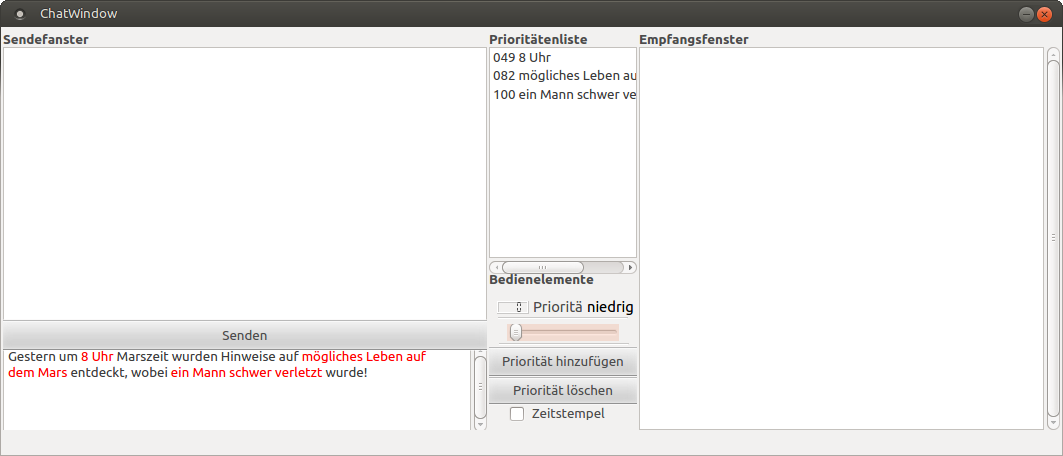
\includegraphics[width=\textwidth]{prioChatWindow.png}
	\label{fig:prioChatWindow}
\end{figure}

Der Text wird jetzt sukzessive, Wort für Wort untersucht und in die
Prioritization-Queue einsortiert (siehe Bild \todo{Bild von ner prio-queue mit
text}). Jedes einzelne Wort bildet dabei einen Datenblock, dem eine
Sequenznummer zugeordnet wird, wodurch eine eindeutige Identifizierung möglich
ist. Die Data Object ID (DOID) beugt einer Verwechslung anderer Datenblöcke,
gleicher Sequenznummer vor. Weiterhin werden die Position und die Länge des
Wortes abgespeichert. Anhand dieser Informationen ist der Empfänger in der Lage
die ankommende Datenblöcke korrekt zuzuordnen und so den Text wieder herzustellen.
Dabei kommen zunächst, wie in Bild MUH \todo{referenz auf bild mit ankommenden
textstücken} zu sehen, die wichtigen, höher priorisierten Textstücke an, gefolgt
von den Niederprioren. 

\begin{figure}[H]
	\centering
	\subfigure{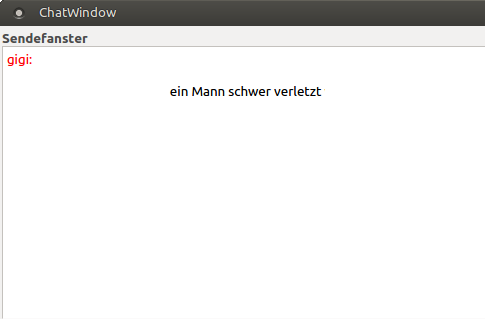
\includegraphics[scale=.4]{chatGuiWindow_empfaenger_prio.png}}\hfill
	\subfigure{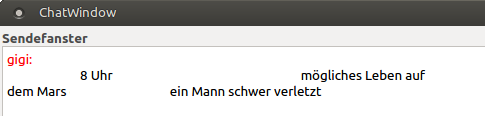
\includegraphics[scale=.4]{chatGuiWindow_empfaenger_halfPrio.png}}\\
	\subfigure{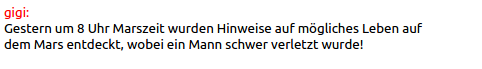
\includegraphics[scale=.4]{chatGuiWindow_empfaenger_all.png}}
	\label{fig:marsWaterResidue}
\end{figure}

Der Ablauf eines Bild gestaltet sich dabei ähnlich. Die Abbildung
\ref{fig:marsWaterResidue} zeigt das vom Marsrover \glqq Curiosity \grqq
am $28.$ September aufgenommene ausgetrocknete Wasserbett. Der im linken Bild
markierte Bereich zeigt, wissenschaftlern zur Folge, einen vom Wasser verformten
Kiesel. Wie beim Szenario zuvor erfolgt zunächst eine Markierung der wichtigen
Bereiche. Hier der Kiesel und der Maßstab (Bild \ref{fig:marsWaterResidue}
mitte). Bevor das Bild wie auch der Text Schritt für Schritt analysiert werden
kann, muss dieser in Abschnitte eingeteilt werden, welche später die einzelnen
Datenblöcke darstellen (Bild \ref{fig:marsWaterResidue}).
 
\begin{figure}[H]
	\centering
	\subfigure{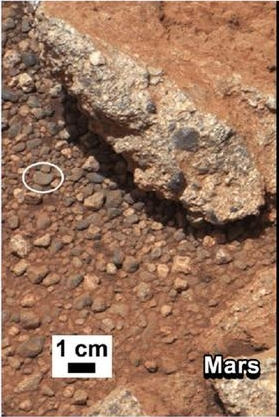
\includegraphics[scale=.4]{marsWaterResidue_links.jpg}}\hfill
	\subfigure{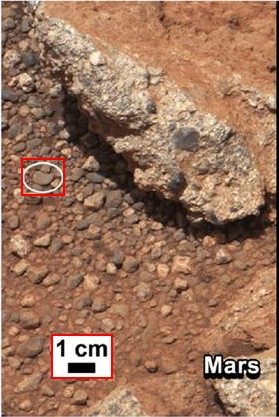
\includegraphics[scale=.4]{marsWaterResidue_mitte.jpg}}\hfill
	\subfigure{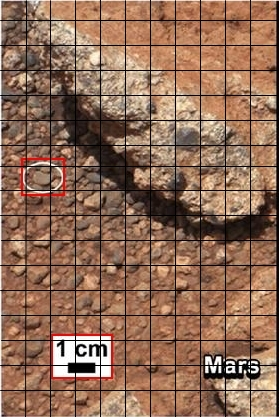
\includegraphics[scale=.4]{marsWaterResidue_rechts.jpg}}
	\label{fig:marsWaterResidue}
\end{figure}

Die weiteren Schritte sind equivalent zu denen des Textes. Die beiden wichtigen
und damit höher priorisierten Bereiche kommen als erstes beim Empfänger an. Das
zusammensetzen des Bildes könnte dann wie in Abbildung
\ref{fig:marsWaterResidueEmpfaenger} zusehen ablaufen.

\begin{figure}[H]
	\centering
	\subfigure{
\includegraphics[scale=.4]{marsWaterResidue_empfaenger_links.jpg}}\hfill
	\subfigure{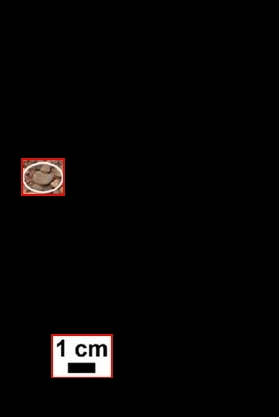
\includegraphics[scale=.4]{marsWaterResidue_empfaenger_mitte.jpg}}\hfill
	\subfigure{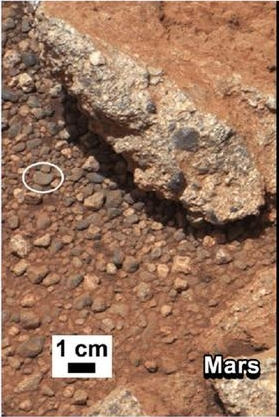
\includegraphics[scale=.4]{marsWaterResidue_empfaenger_rechts.jpg}}
	\label{fig:marsWaterResidueEmpfaenger}
\end{figure}